\documentclass{article}
\usepackage[T1]{fontenc}
\usepackage{lmodern}
\usepackage{graphicx}
\usepackage{amsmath,amssymb}
\usepackage[a4paper,margin=2cm]{geometry}
\usepackage[absolute,overlay]{textpos}
\setlength{\TPHorizModule}{1mm}
\setlength{\TPVertModule}{1mm}
\usepackage[indonesian]{babel}
\usepackage{hyperref}
\setlength{\emergencystretch}{2em}
% unit: Halaman 7

\begin{document}

% === Halaman 7 (llm) ===

\begin{itemize}
  \item \textbf{Case 2:} Bagaimana cara Bob memastikan bahwa pesan tersebut dari Alice dan bukan dari Carol (yang menyamar menjadi Alice)?
\end{itemize}

\vspace{20mm}

\textcolor{red}{Benarkah ini pesan dari Alice?}

\vspace{40mm}

$\rightarrow$ masalah otentikasi (\textit{authentication}) pengirim atau penerima pesan

% deskripsi: Ilustrasi komunikasi pesan antara Alice dan Bob dengan tanda panah yang menunjukkan arah pengiriman pesan.
% bbox normalisasi: [0.2040, 0.3850, 0.7430, 0.6110]
\begin{textblock*}{113.19mm}(42.84mm,114.34mm)
\noindent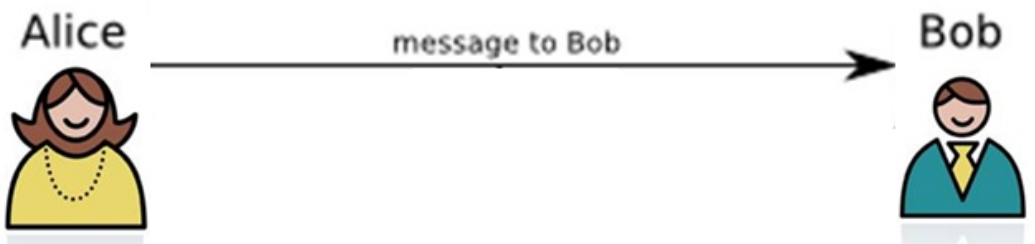
\includegraphics[width=113.19mm,height=67.12mm]{../../images/llm/page_007_img_01.png}%
\end{textblock*}

\end{document}
